% Using template APS for projects
% Commented out non-useful code
% Skyter spurv med kanon

% ****** Start of file apssamp.tex ******
%
%   This file is part of the APS files in the REVTeX 4.1 distribution.
%   Version 4.1r of REVTeX, August 2010
%
%   Copyright (c) 2009, 2010 The American Physical Society.
%
%   See the REVTeX 4 README file for restrictions and more information.
%
% TeX'ing this file requires that you have AMS-LaTeX 2.0 installed
% as well as the rest of the prerequisites for REVTeX 4.1
%
% See the REVTeX 4 README file
% It also requires running BibTeX. The commands are as follows:
%
%  1)  latex apssamp.tex
%  2)  bibtex apssamp
%  3)  latex apssamp.tex
%  4)  latex apssamp.tex
%

\documentclass[%
 reprint,
 nobalancelastpage,
%superscriptaddress,
%groupedaddress,
%unsortedaddress,
%runinaddress,
%frontmatterverbose, 
%preprint,
%showpacs,preprintnumbers,
%nofootinbib,
%nobibnotes,
%bibnotes,
 amsmath,amssymb,
 aps,
%pra,
%prb,
%rmp,
%prstab,
%prstper,
%floatfix,
]{revtex4-1}

\usepackage{graphicx}% Include figure files
\usepackage{dcolumn}% Align table columns on decimal point
\usepackage{hyperref}% add hypertext capabilities
\usepackage{url}% url links
\usepackage{bm}% bold math
\usepackage{booktabs}% tables
\usepackage{listings}% codelisting
\usepackage{subcaption}% create subplots
\usepackage[labelformat=parens,labelsep=quad,skip=3pt]{caption}% caption plots
\usepackage{blindtext}% lorem ipsum...
%\usepackage[mathlines]{lineno}% Enable numbering of text and display math
%\linenumbers\relax % Commence numbering lines

%\usepackage[showframe,%Uncomment any one of the following lines to test 
%%scale=0.7, marginratio={1:1, 2:3}, ignoreall,% default settings
%%text={7in,10in},centering,
%%margin=1.5in,
%%total={6.5in,8.75in}, top=1.2in, left=0.9in, includefoot,
%%height=10in,a5paper,hmargin={3cm,0.8in},
%]{geometry}

\newcommand{\hbarm}{-\frac{\hbar^{2}}{2m}}
\newcommand{\ortwo}{\frac{1}{r^{2}}}
\newcommand{\ddr}{\frac{d}{dr}}
\newcommand{\ddrsq}{\frac{d^{2}}{dr^{2}}}
\newcommand{\ddrhosq}{\frac{d^{2}}{d\rho^{2}}}
\newcommand{\onehalf}{\frac{1}{2}}



\begin{document}

%\preprint{APS/123-QED}

\title{Project 2 - FYS3150}% Force line breaks with \\
\thanks{Computational Physics, autumn 2016, University of Oslo}%

\author{Andreas G. Lefdalsnes}
 % \altaffiliation[Also at ]{Physics Department, XYZ University.}%Lines break automatically or can be forced with \\

% \author{Second Author}%
%  \email{Second.Author@institution.edu}
\affiliation{%
 Student: University of Oslo, Department of Physics\\
 email-address: andregl@student.matnat.uio.no
}%

\author{Tellef Storebakken}
\affiliation{Student: University of Oslo, Department of Physics\\
 email-address: tellefs@student.matnat.uio.no}

% % \collaboration{MUSO Collaboration}%\noaffiliation

% % \author{Charlie Author}
% %  \homepage{http://www.Second.institution.edu/~Charlie.Author}
% % \affiliation{
% %  Second institution and/or address\\
% %  This line break forced% with \\
% % }%
% % \affiliation{
% %  Third institution, the second for Charlie Author
% % }%
% % \author{Delta Author}
% % \affiliation{%
% %  Authors' institution and/or address\\
% %  This line break forced with \textbackslash\textbackslash
% % }%

% % \collaboration{CLEO Collaboration}%\noaffiliation

\date{\today}% It is always \today, today,
             %  but any date may be explicitly specified

\begin{abstract}
In this project we solve the Schrodinger equation for two electrons in a 3D harmonic oscillator potential. We solve with and without electron repulsion, and compare the results. To accomplish this we apply a general method of discretizing the domain and reducing the problem to an eigenvalue equation. We thereafter apply Jacobi's rotation algorithm to obtain the eigenvalues of the matrix. We also apply the principles of unit testing by testing the algorithm for some simple problems with known solutions.

% % An article usually includes an abstract, a concise summary of the work
% % covered at length in the main body of the article. 
% % \begin{description}
% % \item[Usage]
% % Secondary publications and information retrieval purposes.
% % \item[PACS numbers]
% % May be entered using the \verb+\pacs{#1}+ command.
% % \item[Structure]
% % You may use the \texttt{description} environment to structure your abstract;
% % use the optional argument of the \verb+\item+ command to give the category of each item. 
% % \end{description}
\end{abstract}

% % \pacs{Valid PACS appear here}% PACS, the Physics and Astronomy
% %                              % Classification Scheme.
% % %\keywords{Suggested keywords}%Use showkeys class option if keyword
% %                               %display desired

\maketitle

\section{\label{sec:Int}Introduction}
In this project we aim to solve the Schrodinger equation for two electrons in a 3D harmonic oscillator potential. We will be solving with and without the repulsive Coulomb potential, and comparing the results. For the case of no repulsion we have an analytical expression for the energies, and this will be useful in determining the accuracy of our results. Assume spherical symmetry.

\section{\label{sec:The}Theory and methods}

\subsection{\label{sec:Rad}The radial equation}
We begin by studying the radial part of Schrodingers' equation for a single electron in a harmonic oscillator potential \footnote{All theory in this project adapted from FYS3150 Project 2 (Fall 2016) $\href{https://github.com/CompPhysics/ComputationalPhysics/tree/master/doc/Projects/2016/Project2}{<link>}$}.

\begin{equation}
	\hbarm	(\ortwo \ddr r^{2} - \frac{l(l+1)}{r^{2}}) R(r) + V(r)R(r) = E R(r)
\end{equation}

The potential $V(r) = \onehalf kr^{2}$ is the harmonic oscillator potential with $k = m\omega^{2}$ and E is the energy of the electron. $\omega$ is the oscillator frequency and the allowed energies are

\begin{equation}
	E_{nl} = \hbar \omega (2n+l+\frac{3}{2})
\end{equation}

Where the quantum number $n = 0,1,2..$ is the energy quantum number and $l = 0,1,2...$ is the orbital momentum quantum number. Introducing $R(r) = (1/r)u(r)$ our equation can be rewritten in terms of the second derivative $d^{2}/dr^{2}$:

\begin{equation}
	\hbarm \ddrsq u(r) + (V(r) + \frac{l(l+1)}{r^{2}}\hbarm)u(r) = Eu(r)
\end{equation}
\\
We introduce a dimensionless variable $\rho = (1/ \alpha)r$ where alpha is a constant of dimension length and obtain

\begin{equation}
	-\frac{\hbar^{2}}{2m\alpha^{2}} \ddrhosq u(\rho) + (V(\rho) + \frac{l(l+1)}{\rho^{2}}\frac{\hbar^{2}}{2m\alpha^{2}})u(\rho) = E u(\rho)
\end{equation}

In this project we will be interested in the case $l = 0$. Now since we are working in spherical coordinates, $r \in [0, \infty)$. Since we require $R(r)$ to go to zero at the boundaries, when we make the substituion $R(r) = (1/r)u(r) = (1/r)u(\alpha \rho)$ we obtain the boundary conditions for $u(\rho)$: $u(0) = u(\infty) = 0$.
\\ \\
We insert $V(\rho) = \onehalf k\alpha^{2}\rho^{2}$ and obtain

\begin{equation}
	-\frac{\hbar^{2}}{2m\alpha^{2}} \ddrhosq u(\rho) + \onehalf k\alpha^{2} \rho^{2}u(\rho) = E u(\rho)
\end{equation}

To obtain a simpler expression we multiply by $2m\alpha^{2} \rho^{2} /\hbar^{2}$ and fix $\alpha$ such that

\begin{equation}
	\frac{mk}{\hbar^{2}}\alpha^{4} = 1
\end{equation}

and define

\begin{equation}
	\lambda = \frac{2m\alpha^{2}}{\hbar^{2}}E
\end{equation}

so we can rewrite our equation as

\begin{equation}
	-\ddrhosq u(\rho) + \rho^{2} u(\rho) = \lambda u({\rho})
\end{equation}

To solve this equation we discretize the domain and define minimum and maximum values for $\rho$, $\rho_{min} = \rho_{0} = 0$ and $\rho_{max}$. $\rho_{max}$ cannot be chosen to be $\infty$ so we must take care to set it sufficiently large in order to obtain the correct solution. With $N$ mesh points let

\begin{equation}
	h = \frac{\rho_{max}-\rho_{0}}{N}
\end{equation}

and we obtain a discrete set of values for $\rho$, 

\begin{equation}
	\rho_{i} = \rho_{0} + ih \qquad i=0,1,2...,N
\end{equation}

Replacing the second order derivative by the 2nd order central difference we can write our equation as 

\begin{equation}
	-\frac{u_{i+1}+u_{i-1}-2u_{i}}{h^{2}} + \rho_{i}^{2}u_{i} = \lambda u_{i}
\end{equation}

Where $u_{i} = u(\rho_{i})$ is the discretized version of our function. We let $V_{i} = \rho_{i}^{2}$ and rewrite this as a matrix equation

\begin{equation}
	\bm{Au} = \lambda\bm{u}
\end{equation}

Since the endpoints are known we let $A$ be a matrix of dimension $(n-2)\cdot(n-2)$ and $u$ a vector of dimension (n-2).


\begin{widetext}
\begin{equation}
\bm{Au} =
\begin{pmatrix}
  \frac{2}{\hbar^{2}} + V_{1} & -\frac{1}{\hbar^{2}} & 0 & \cdots & \cdots & 0 \\
  -\frac{1}{\hbar^{2}} & \frac{2}{\hbar^{2}} + V_{2} &  -\frac{1}{\hbar^{2}} & 0 &\cdots & \cdots \\
  0 & -\frac{1}{\hbar^{2}} & \frac{2}{\hbar^{2}} + V_{3} & -\frac{1}{\hbar^{2}} & 0 & \cdots \\
  \vdots & \vdots & \vdots & \vdots & \vdots & \vdots \\
  0 & \cdots & \cdots & -\frac{1}{\hbar^{2}} & \frac{2}{\hbar^{2}} + V_{N-3} & -\frac{1}{\hbar^{2}} \\
  0 & \cdots & \cdots & \cdots & -\frac{1}{\hbar^{2}} & \frac{2}{\hbar^{2}} + V_{N-2}
\end{pmatrix}
\begin{pmatrix}
	u_{1} \\
	u_{2} \\
	\vdots \\
	\\
	\\
	u_{N-2}
\end{pmatrix}
=	\lambda
\begin{pmatrix}
	u_{1} \\
	u_{2} \\
	\vdots \\
	\\
	\\
	u_{N-2}
\end{pmatrix}
\end{equation}
\end{widetext}

where $u_{0} = u_{N-1} = 0$.

\subsection{Coulomb Interaction}
For two electrons with no Coulomb interaction in a harmonic oscillator potential the Schroedinger equation can be written as

\begin{equation}
	(\hbarm \frac{d^{2}}{dr_{1}^{2}} \hbarm \frac{d^{2}}{dr_{2}^{2}} + \onehalf k r_{1}{2} + k r_{2}^2)u(r_{1}, r_{2}) = Eu(r_{1}, r_{2})
\end{equation}

With no interaction the two-electron wavefunction $u(r_{1}, r_{2})$ can be written as a product of two single-electron wavefunction. Introducing the relative coordinate $\bm{r} = \bm{r_{1} - r_{2}}$ and the center of mass coordinate $\bm{R} = \onehalf (\bm{r_{1} + r_{2}})$ the radial equation becomes

\begin{equation}
	(-\frac{\hbar^{2}}{m}\frac{d^{2}}{dr^{2}} - \frac{\hbar^{2}}{4m} \frac{d^{2}}{dR{2}} + \frac{1}{4}kr^{2} + kR^{2}) u(r, R) = Eu(r, R)
\end{equation}

the solution can be separated as $u(r, R) = \psi(r)\phi(R)$ and the energy is a sum of the relative energy $E_{r}$ and center-of-mass energy $E_{R}$

\begin{equation}
	E = E_{r} + E_{R}
\end{equation}

adding the repulsive Coulomb interaction

\begin{equation}
	V(r_{1}, r_{2}) = \frac{\beta e^{2}}{\left| \bm{r_{1}-r_{2}} \right|} = \frac{\beta e^{2}}{r}
\end{equation}

where $\beta e^{2}  = 1.44$ eVnm. The relative motion Schroedinger equation becomes

\begin{equation}
	(-\frac{\hbar^{2}}{m}\frac{d^{2}}{dr^{2}} + \frac{1}{4}kr^{2} + \frac{\beta e^{2}}{r}) \psi(r) = E\psi(r)
\end{equation}

introducing $\rho = r/\alpha$, defining a new frequency

\begin{equation}
	\omega_{r}^{2} = \frac{1}{4} \frac{mk}{\hbar^{2}} \alpha^{4}
\end{equation}

fixing $\alpha$

\begin{equation}
	\alpha \frac{m \beta e^{2}}{\hbar^{2}} = 1
\end{equation}

and defining

\begin{equation}
	\lambda = \frac{m\alpha^{2}}{\hbar^{2}} E
\end{equation}

and we obtain Schroedinger's equation

\begin{equation}
	-\ddrhosq \psi(\rho) + \omega_{r}^{2}\rho^{2}\psi(\rho) + \frac{1}{\rho} = \lambda \psi(\rho)
\end{equation}

which using the methods described in the previous section can be solved numerically as an eigenvalue problem.

\subsection{Jacobi's rotation method}
For a real symmetric $n\cdot n$ matrix $\bm{A}$, we have $n$ eigenvalues $\lambda_{i}$ and there exists a real orthogonal matrix $\bm{S}$ such that 
\footnote{See M.H. Jensen, Computational Physics: Lecture Notes Fall 2015, ch. 7.3, available at $\href{https://github.com/CompPhysics/ComputationalPhysics/blob/master/doc/Lectures/lectures2015.pdf}{<link2>}$}

\begin{equation}
	\bm{S^{T}AS} = diag(\lambda_{1}, \lambda_{2},...,\lambda_{n})
\end{equation}

In general a similarity transform

\begin{equation}
	\bm{B = S^{T}AS} \qquad \qquad \bm{S^{T}S = I}
\end{equation}

will have the same eigenvalues as $\bm{A}$, but different eigenvectors. If we have an orthogonal basis $v_{i}$ such that

\begin{equation}
	\bm{v_{j}^{T}v_{i} = \delta_{ij}}
\end{equation}

a unitary transformation $\bm{U^{T}U = I}$ will preserve the orthogonality of the basis vectors, such that if $w_{i} = Uv_{i}$

\begin{equation}
	\bm{w_{j}^{T}w_{i} = (Uv_{j})^{T}(Uv_{i}) = v_{j}^{T}U^{T}Uv_{i} = \delta_{ij}}
\end{equation}

The idea of Jacobi's method is to perform a series of similarity transformations such that we receive a diagonal matrix $\bm{D}$ with the eigenvalues of $\bm{A}$ on the diagonal. \\ \\
Consider a $N\times N$ matrix

\begin{equation}
S = 
	\begin{pmatrix}
		1 & 0 & \cdots & 0 & 0 \cdots & 0 & 0 \\
		0 & 1 & \cdots & 0 & 0 \cdots & 0 & 0 \\
		\cdots & \cdots & \cdots & \cdots & \cdots & 0 & \cdots \\
		0 & 0 & \cdots & \cos(\theta) & 0 \cdots & 0 & \sin(\theta) \\
		0 & 0 & \cdots & 0 & 1 \cdots & 0 & 0 \\
		\cdots & \cdots & \cdots & \cdots & \cdots & 0 & \cdots \\
		0 & 0 & \cdots & 0 & 0 \cdots & 1& 0 \\
		0 & 0 & \cdots & -\sin(\theta) & 0 \cdots & 0 & \cos(\theta) \\	
	\end{pmatrix}
\end{equation}

with $\bm{S^{T} = S^{-1}}$. It performs a plane rotation around an angle $\theta$ in $n$-dimensional space. We apply a similarity transformation $\bm{S^{T}AS}$ to our matrix $\bm{A}$ such that the largest non-diagonal elements $a_{kl} = a_{lk}$ become zero. For a real symmetric matrix we thus reduce the norm of the offdiagonal elements

\begin{equation}
	\text{off}(\bm{A}) = \sqrt{\sum_{i=1}^{n}\sum_{j=1, j\neq i}^{n}} a_{ij}^{2}
\end{equation}

and after a sufficient number of iterations we are guaranteed a matrix

\begin{equation}
	\bm{S_{N}^{T}S_{N-1}^{T}....S_{1}^{T}AS_{1}....S_{N-1}S_{N} = diag(\lambda_{1},...,\lambda_{N})}
\end{equation}

Numerically it is sufficient that the largest non-diagonal element is smaller than some tolerance $\epsilon$

\begin{equation}
	max(a_{ij}^{2}) \leq \epsilon
\end{equation}

Convergence is guaranteed with the Jacobi method, however the number of floating point operations is quite large, $\mathcal{O}(12n^{3})$ operations in order to zero out non-diagonal elements.

%<<<<<<< HEAD
%\subsection{Tests}
%
%We were to implement some unit-tests in to our program. In our progam we had a function to find the largest element of the diagonal, called $maxOffDiag$. In the test we sent in a $3x3$ matrix where we know the largest element of the diagonal, and checks of our function $maxOffDiag$ returns the right element.\\
%Our other test was to check of the eigenvector we got was orthogonal which they should be. Here we just computed the dot-product between all the resulting eigenvectors and checked of the value was lower than a decided tolerance. We set the tolerance to be $tol = 10^{-5}$.
%=======
\subsection{Unit testing}
In order to test the accuracy of our methods we can introduce some simple unit tests. For example we could check that our implementation of Jacobi's method for a simple symmetric matrix with known eigenvalues produces the exact results. For our problem the 3 lowest eigenvalues are known in the case of no interaction, and it is easy to test for example if our algorithm produces the lowest eigenvalue to some precision. \\
In addition, the solutions to the Schroedinger equation form an orthogonal basis. In the previous subsection I show that an orthogonal transformation preserves orthogonality, so we can test our algorithm by checking to see if the resulting eigenvectors are orthogonal.\\
Finally, we test our function to find the maximum off-diagonal value of a matrix by testing it on a simple 3x3 symmetric matrix.
%>>>>>>> 73d3c01504e8fb9524d03c3179d3c9bcaef5b424


\section{RESULTS AND DISCUSSION}

\subsection{Programming precision}
% In the case of no electron interaction we know exactly the lowest 3 eigenvalues of the matrix $A$. To find the lowest eigenvalue $\lambda = 3$ we require roughly $N = 200$ mesh points to obtain an accuracy of $\left| \lambda - \lambda_{num} \right| \approx 0.0002$.


First we checked how many mesh points $N$ we needed. We ran the program for a system where we knew the lowest eigenvalue and wanted the difference to be less than $10^{-4}$. When doing this for a known problem where the lowest eigenvalue should have been $\lambda_{theory} = 3$ we found that we needed $N=200$ mesh points to get this precision.\\
We also checked how many similarity transformations we needed before all the non-diagonal elements were essentially zero. In the program we checked this by adding a counter which checked how many times we rotated matrix elements. We found that with $N= 200$ mesh points, we needed approximately $66600$ transformations. Our tolerance when doing this was that the diagonal elements had to be lower than $tol = 10^{-8}$.\\

Now that we found our right mesh point precision, we timed our algorithm and compared it to the $c++$ library Armadillo. In Table (1) the times are included.

\begin{table}[h]
\centering
\caption{Time comparison}
\label{my-label}
\begin{tabular}{|l|l|}
\hline
\textbf{Method}  & \textbf{Time {[}s{]}} \\ \hline
Jacobi algorithm & $13.73$               \\ \hline
Armadillo        & $0.02$                \\ \hline
\end{tabular}
\end{table}

From Table (1) we can see that the method we have used for finding the eigenvalues is very inefficient compared to the method Armadillo is using. We have then used the armadillo-function $eig\_ sym(A)$ which also solves for a symmetric matrix $A$ just like we have done in our Jacobi-method. The difference is while we assume the whole matrix is filled with elements, $eig\_sym$ takes advantage of the fact that we have a sparse matrix (we have a tridiagonal matrix where the rest of the elements are zeros).

\subsection{Coulomb interaction}
In this project we were interested in the ground state energies. In the program, this would mean the eigenvector that corresponds to the lowest eigenvalue. Since we were only interested in the lowest state, and not the second-lowest etc. this was pretty straight forward.\\

Now we will compare the ground-statre energies for the case where the electrons are interacting and when they are not interacting, for different values of $\omega_R$ (see figure (1), (2), (3), and (4)). We can see that for low values of $\omega_R$ the interacting case gives a wider wave-function (figure (1)). For higher $\omega_R$ the interacting and the non-interacting case gets closer (figure (2) and (3)), but when $\omega_R$ gets higher than $1$ they start to differ again. We can see that for $\omega_R = 5$ (figure (4)) the non-interacting case gets a narrower wave-function. This means that for higher $\omega_R$'s it will be easier to locate the electrons i.e. the probability to find them is higher. \\
These results means that the $\omega_R$ factor has more to say than the Coulomb-interaction $\frac{1}{\rho}$ (see Equation (22)) when changing the $\omega_R$ factor. We can see this from Figure (3) where $\oemga_R = 1$. This is the case where the wave-functions are most similar compared to the other plots (figure (1), (2), and (4)).

 \begin{figure}[h]
\centering
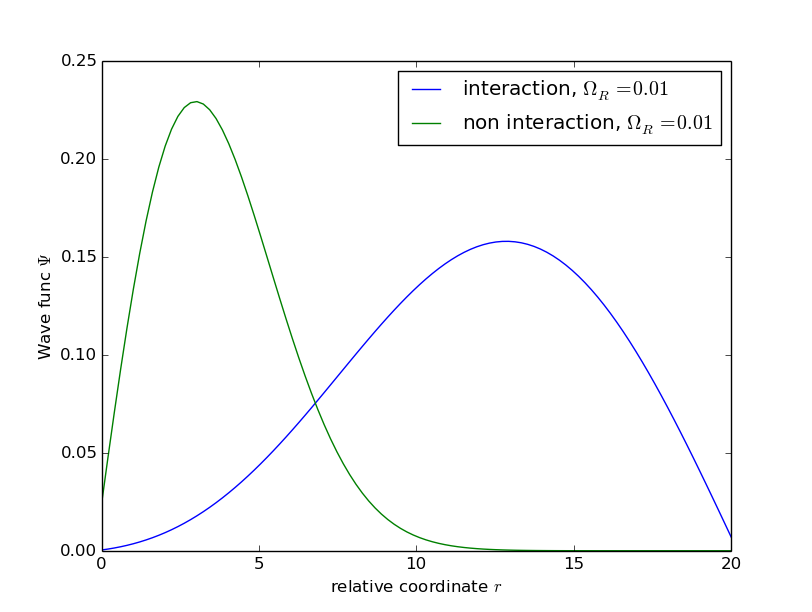
\includegraphics[width=0.5\textwidth]{../omega001.png}
\caption{•}
\label{fig:my_label}
\end{figure}

 \begin{figure}[h]
\centering
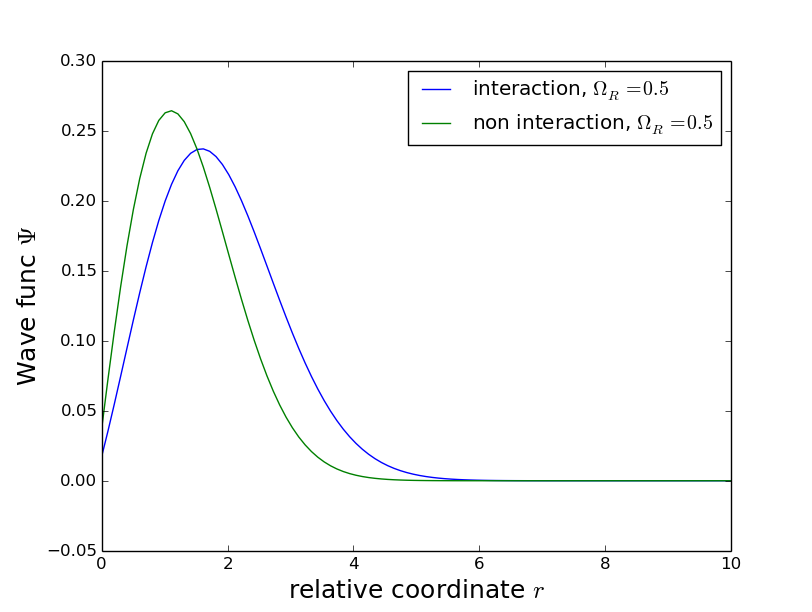
\includegraphics[width=0.5\textwidth]{../omega05.png}
\caption{•}
\label{fig:my_label}
\end{figure}

 \begin{figure}[h]
\centering
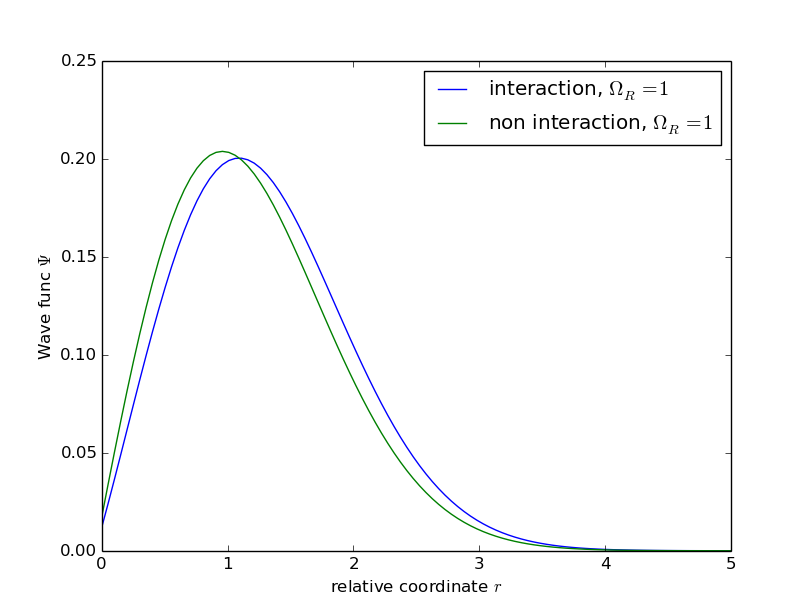
\includegraphics[width=0.5\textwidth]{../omega1.png}
\caption{•}
\label{fig:my_label}
\end{figure}

 \begin{figure}[h]
\centering
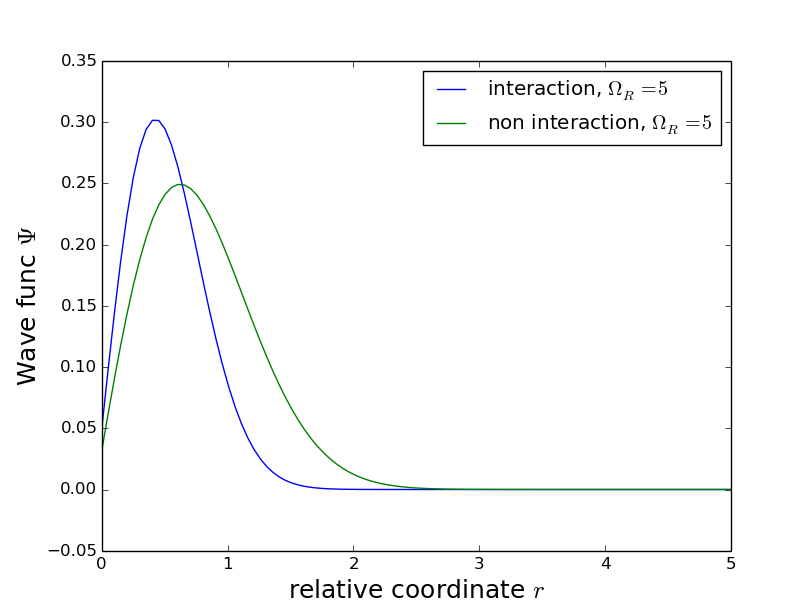
\includegraphics[width=0.5\textwidth]{../omega5.png}
\caption{•}
\label{fig:my_label}
\end{figure}




%\tableofcontents 

% \section{\label{sec:level1}First-level heading}

% This sample document demonstrates proper use of REV\TeX~4.1 (and
% \LaTeXe) in mansucripts prepared for submission to APS
% journals. Further information can be found in the REV\TeX~4.1
% documentation included in the distribution or available at
% \url{http://authors.aps.org/revtex4/}.

% When commands are referred to in this example file, they are always
% shown with their required arguments, using normal \TeX{} format. In
% this format, \verb+#1+, \verb+#2+, etc. stand for required
% author-supplied arguments to commands. For example, in
% \verb+\section{#1}+ the \verb+#1+ stands for the title text of the
% author's section heading, and in \verb+\title{#1}+ the \verb+#1+
% stands for the title text of the paper.

% Line breaks in section headings at all levels can be introduced using
% \textbackslash\textbackslash. A blank input line tells \TeX\ that the
% paragraph has ended. Note that top-level section headings are
% automatically uppercased. If a specific letter or word should appear in
% lowercase instead, you must escape it using \verb+\lowercase{#1}+ as
% in the word ``via'' above.

% \subsection{\label{sec:level2}Second-level heading: Formatting}

% This file may be formatted in either the \texttt{preprint} or
% \texttt{reprint} style. \texttt{reprint} format mimics final journal output. 
% Either format may be used for submission purposes. \texttt{letter} sized paper should
% be used when submitting to APS journals.

% \subsubsection{Wide text (A level-3 head)}
% The \texttt{widetext} environment will make the text the width of the
% full page, as on page~\pageref{eq:wideeq}. (Note the use the
% \verb+\pageref{#1}+ command to refer to the page number.) 
% \paragraph{Note (Fourth-level head is run in)}
% The width-changing commands only take effect in two-column formatting. 
% There is no effect if text is in a single column.

% \subsection{\label{sec:citeref}Citations and References}
% A citation in text uses the command \verb+\cite{#1}+ or
% \verb+\onlinecite{#1}+ and refers to an entry in the bibliography. 
% An entry in the bibliography is a reference to another document.

% \subsubsection{Citations}
% Because REV\TeX\ uses the \verb+natbib+ package of Patrick Daly, 
% the entire repertoire of commands in that package are available for your document;
% see the \verb+natbib+ documentation for further details. Please note that
% REV\TeX\ requires version 8.31a or later of \verb+natbib+.

% \paragraph{Syntax}
% The argument of \verb+\cite+ may be a single \emph{key}, 
% or may consist of a comma-separated list of keys.
% The citation \emph{key} may contain 
% letters, numbers, the dash (-) character, or the period (.) character. 
% New with natbib 8.3 is an extension to the syntax that allows for 
% a star (*) form and two optional arguments on the citation key itself.
% The syntax of the \verb+\cite+ command is thus (informally stated)
% \begin{quotation}\flushleft\leftskip1em
% \verb+\cite+ \verb+{+ \emph{key} \verb+}+, or\\
% \verb+\cite+ \verb+{+ \emph{optarg+key} \verb+}+, or\\
% \verb+\cite+ \verb+{+ \emph{optarg+key} \verb+,+ \emph{optarg+key}\ldots \verb+}+,
% \end{quotation}\noindent
% where \emph{optarg+key} signifies 
% \begin{quotation}\flushleft\leftskip1em
% \emph{key}, or\\
% \texttt{*}\emph{key}, or\\
% \texttt{[}\emph{pre}\texttt{]}\emph{key}, or\\
% \texttt{[}\emph{pre}\texttt{]}\texttt{[}\emph{post}\texttt{]}\emph{key}, or even\\
% \texttt{*}\texttt{[}\emph{pre}\texttt{]}\texttt{[}\emph{post}\texttt{]}\emph{key}.
% \end{quotation}\noindent
% where \emph{pre} and \emph{post} is whatever text you wish to place 
% at the beginning and end, respectively, of the bibliographic reference
% (see Ref.~[\onlinecite{witten2001}] and the two under Ref.~[\onlinecite{feyn54}]).
% (Keep in mind that no automatic space or punctuation is applied.)
% It is highly recommended that you put the entire \emph{pre} or \emph{post} portion 
% within its own set of braces, for example: 
% \verb+\cite+ \verb+{+ \texttt{[} \verb+{+\emph{text}\verb+}+\texttt{]}\emph{key}\verb+}+.
% The extra set of braces will keep \LaTeX\ out of trouble if your \emph{text} contains the comma (,) character.

% The star (*) modifier to the \emph{key} signifies that the reference is to be 
% merged with the previous reference into a single bibliographic entry, 
% a common idiom in APS and AIP articles (see below, Ref.~[\onlinecite{epr}]). 
% When references are merged in this way, they are separated by a semicolon instead of 
% the period (full stop) that would otherwise appear.

% \paragraph{Eliding repeated information}
% When a reference is merged, some of its fields may be elided: for example, 
% when the author matches that of the previous reference, it is omitted. 
% If both author and journal match, both are omitted.
% If the journal matches, but the author does not, the journal is replaced by \emph{ibid.},
% as exemplified by Ref.~[\onlinecite{epr}]. 
% These rules embody common editorial practice in APS and AIP journals and will only
% be in effect if the markup features of the APS and AIP Bib\TeX\ styles is employed.

% \paragraph{The options of the cite command itself}
% Please note that optional arguments to the \emph{key} change the reference in the bibliography, 
% not the citation in the body of the document. 
% For the latter, use the optional arguments of the \verb+\cite+ command itself:
% \verb+\cite+ \texttt{*}\allowbreak
% \texttt{[}\emph{pre-cite}\texttt{]}\allowbreak
% \texttt{[}\emph{post-cite}\texttt{]}\allowbreak
% \verb+{+\emph{key-list}\verb+}+.

\end{document}
%
% ****** End of file apssamp.tex ******